\chapter{Results}  \label{sec:results}


\section{Experiments}  \label{sec:experiments}

To evaluate the effectiveness of the previously defined \ac{dea}, a series of experiments are conducted using multiple datasets.
These experiments aim to assess the attack's performance across different encoding schemes and datasets using different execution settings to analyze its ability to reconstruct plaintext information from encoded identifiers.

The primary dataset used is the \texttt{fakename} dataset, which is synthetically generated using the American name set provided by the Fake Name Generator.
This dataset was previously employed in related work by Schaefer et al.~\cite{schaefer2024}, making it a suitable benchmark for comparative evaluation.
It includes realistic combinations of personal identifiers and is well-suited for testing the scalability and reliability of both the \ac{gma} and \ac{dea} pipelines.

The \texttt{fakename} datasets consist of synthetically generated entries, each containing a given name, surname, and date of birth.
These datasets aim to resemble realistic combinations of personal identifiers while ensuring privacy and reproducibility.
For evaluation purposes, multiple dataset instances of varying sizes are used: 1{,}000, 2{,}000, 5{,}000, 10{,}000 and 20{,}000 entries.

The primary advantage of using this dataset family lies in its scalability.
By maintaining a consistent schema while varying the number of records, the impact of dataset size on the performance and success of the \ac{dea} can be systematically analyzed.
This enables controlled experiments that highlight how the quantity of available data influences re-identification, training quality, and generalization performance of the attack models.

An additional dataset used in this study is the \texttt{euro\_person} dataset provided as part of the simulated data for the ESSnet DI on-the-job training course on record linkage.
The dataset was created by Paula McLeod, Dick Heasman, and Ian Forbes from the UK Office for National Statistics and contains realistic, fictionalized personal information intended for the training and evaluation of record linkage techniques.
The \texttt{euro\_person} dataset includes forename (\texttt{PERNAME1}), surname (\texttt{PERNAME2}), and full date of birth composed of day, month, and year, which were concatenated into a single \texttt{DOB\_FULL} attribute for the purposes of this work.
The dataset consisting of 26.625 records also serves as a ground-truth reference for other simulated sources such as Census, CIS, and PRD, it is well-suited for evaluating the precision and completeness of plaintext reconstruction and re-identification in the context of the \ac{dea}.

In addition to the synthetic and benchmark datasets, this thesis also incorporates a curated version of the Titanic passenger manifest, referred to as \texttt{titanic\_full}.
This dataset consists of 891 unique records and includes the fields \texttt{firstname} and \texttt{surname}.
While not originally intended for record linkage evaluation, the dataset offers a semi-realistic collection of personal identifiers derived from historical records.
It provides a useful case for examining the impact of natural name diversity, varying name lengths, and non-standard naming formats (e.g., inclusion of titles or parenthetical information) on the performance of both \ac{gma} and \ac{dea}.
Due to the historical and English centric nature of the data, it shares some limitations with other Western-focused datasets used in this work but nonetheless adds valuable variety in terms of name structure and frequency.

The experiments are conducted across a range of settings and scenarios to comprehensively evaluate the effectiveness of the \ac{dea}.
Each encoding scheme, namely \ac{bf}, \ac{tsh}, and \ac{tmh}, is tested individually across all datasets as described earlier.
This allows for a direct comparison of reconstruction performance under different privacy-preserving encoding mechanisms.

To ensure consistent and comparable evaluation across all encoding schemes, standardized configuration parameters were employed for both Alice's and Eve's encoding processes.
All three encoding schemes used 2-grams with Dice similarity as the distance metric, providing a common baseline for structural comparison.
For \ac{bf} encoding, both parties used a filter length of 1024 bits with 10 hash functions and no diffusion layer, ensuring maximum compatibility while maintaining reasonable privacy guarantees.
\ac{tmh} configurations employed 1024 hash functions with 64-bit precision, 8 sub-keys, and 1-bit hash output, balancing computational efficiency with encoding quality.
\ac{tsh} settings utilized 10 hash functions with 1000 columns and \ac{prng}-based randomization, providing sufficient dimensionality for effective similarity preservation.
These standardized parameters ensure that performance differences observed in the experiments can be attributed to the fundamental characteristics of each encoding scheme rather than configuration-specific optimizations.

To additionally analyze how the quantity of the training data affects the \ac{dea}, the preceding \ac{gma} step is executed with varying levels of overlap between Alice's and Eve's datasets.
For each dataset and encoding scheme, the \ac{gma} is run multiple times with overlap ratios ranging from 20\% to 80\%, in increments of 20\%.
This simulates different real world scenarios where the attacker has access to varying amounts of auxiliary information.
The resulting re-identifications from the \ac{gma} then serve as the labeled training data for the \ac{dea}, thus allowing for a detailed evaluation of how overlap levels influence overall reconstruction success.

In addition to varying dataset sizes and overlap levels, different attacker scenarios are considered by employing different drop from strategies to evaluate the robustness of the \ac{dea} under more and less realistic assumptions.
The first scenario, Eve's auxiliary dataset $D_p$ is a strict subset of Alice's dataset $D_e$, i.e., $D_p \subseteq D_e$.
In this case, the overlap $o$ is defined as the ratio $o = \frac{|D_p|}{|D_e|}$.
The elements in $D_p$ are generated by randomly sampling $|D_p| = \lfloor o \cdot |D_e| \rfloor$ records from $D_e$ without replacement.
While this setup simplifies evaluation and isolates the impact of training data availability, it is also highly idealized and does not reflect the complexity of real world linkage scenarios.

To address this, a second, more realistic setting is also considered, where both $D_p$ and $D_e$ contain disjoint as well as overlapping individuals.
That is, $D_e \nsubseteq D_p$, but $D_e \cap D_p \neq \emptyset$.
In this scenario, the auxiliary and target datasets each include individuals not present in the other, simulating cases where Eve has partial but non exclusive knowledge of the data.
This setup introduces additional challenges for both the \ac{gma} and \ac{dea}, as structural mismatches and auxiliary noise may degrade re-identification and reconstruction accuracy.

This setup mirrors the experimental methodology employed by \cite{schaefer2024}, ensuring consistency and comparability with prior work on the \ac{gma}.
By varying the overlap rate and dataset composition in this way, a diverse range of re-identification scenarios is created, which directly impacts the amount and quality of training data available for the \ac{dea}.
This, in turn, enables a systematic evaluation of the \ac{dea}'s ability to generalize from partially re-identified data.

As the \ac{gma} identifies different subsets of individuals under varying overlap conditions, the resulting re-identification sets are used to train the neural network, while the remaining non matched records serve as the test set.
Thus, each experiment yields a distinct train-test split, providing a rich basis for assessing the reconstruction capabilities of the \ac{dea}.

For the \ac{dea} specific configuration, several fixed settings were employed to ensure comparability across all experimental conditions.
First, the dataset of re-identified individuals, used as labeled training data, was split into training and validation sets using a fixed 80/20 ratio.
This choice reflects common \ac{ml} practice and provides a balanced compromise between model learning and validation reliability.

One of the most critical components of the \ac{dea} pipeline is the hyperparameter optimization step, which is responsible for identifying the most effective neural network architecture.
For this purpose, a total of 125 trials were conducted for each experimental setting.
This number was chosen to provide sufficient coverage of the hyperparameter space while maintaining computational feasibility.

Each trial, as well as the final training run for the best performing model, was limited to a maximum of 20 training epochs.
While this represents a relatively high upper bound, overfitting is mitigated through the use of early stopping.
Specifically, training was halted if the validation loss did not improve for five consecutive epochs (patience = 5), with a minimum delta of $1 \cdot 10^{-4}$ required to qualify as an improvement.
This strategy ensures both efficient training and effective model selection, especially when performance plateaus early.

The search space for the hyperparameter optimization follows the configuration described in Section~\ref{sec:hmo}.
Throughout the entire \ac{dea} pipeline, the \textbf{Dice coefficient} is used as the objective metric for optimization.
This choice is motivated by its robustness and balanced nature, as it integrates both precision and recall and has consistently yielded the most promising results during preliminary manual testing.

For efficient optimization, the hyperparameter search is executed using all available CPU cores.
Additionally and optionally an NVIDIA GPU can be used to accelerate the training of the neural networks during hyperparameter optimization.
This allows for near maximal parallelism during hyperparameter tuning, reducing the total runtime of the experiments.

In the final re-identification phase, two reconstruction strategies are evaluated to enable comparative analysis: (1) the greedy, graph-based reconstruction method described in Section~\ref{sec:graphrecon}, and (2) the dictionary-based fuzzy matching approach described in Section~\ref{sec:dictrecon}.
Both methods are deterministic and computationally efficient, making them suitable for large scale experimental evaluation.

The language model based reconstruction method is excluded from the evaluation.
Despite showing potential in early qualitative testing, its dependence on external models, token-based pricing, and limited reproducibility make it unsuitable for scalable and reproducible experimentation within the current research setting.

All experiments were conducted on a virtual machine running Ubuntu 24.04, equipped with 20 cores of a virtualized AMD processor (QEMU Virtual CPU).
The system was provisioned with 176 GB of RAM and featured an NVIDIA GeForce RTX 3090 Ti GPU with 24 GB of dedicated VRAM.

This high-performance computing setup enabled efficient parallel execution of the hyperparameter optimization trials and accelerated training of the neural networks via GPU.
The extensive memory capacity was particularly beneficial during dataset preprocessing and batch-wise loading of large datasets, ensuring that all encoding schemes and reconstruction strategies could be evaluated without resource bottlenecks.


\section{Evaluation Metrics}  \label{sec:metrics}

The performance of the \ac{dea} is assessed using several metrics that are systematically recorded throughout the experimental runs.

Although the \ac{dea} constitutes an offline attack, meaning the attacker can operate without time constraints once both encoded datasets are available, the runtime of the attack remains a valuable indicator of its practical feasibility.
Therefore, the total runtime as well as the runtime of each individual stage within the \ac{dea} pipeline (e.g., data preprocessing, model training, hyperparameter optimization, inference, and reconstruction) is measured and documented.

A central metric for assessing the effectiveness of the attack is the \emph{re-identification rate}.
This metric is defined as the number of individuals that are successfully and correctly re-identified by the \ac{dea}, divided by the total number of individuals who were not matched during the initial \ac{gma}.

A successful re-identification in this context means that the \ac{dea} is able to fully reconstruct the original plaintext attributes of a record such that it exactly matches a record in Alice's encoded dataset.
Thus, the re-identification rate reflects the proportion of previously unmapped individuals that the attacker can recover using the inference based approach.

Another important aspect of evaluating the \ac{dea} is its performance in predicting the correct n-grams, which forms the basis for reconstructing plaintext attributes.
To assess the quality of these predictions, several standard classification metrics are considered, namely, precision, recall, and the F1-score.

In the context of this work, the F1-score is of particular interest, as it has shown to be the most reliable metric for quantifying n-gram-level performance.
Moreover, it is mathematically equivalent to the Dice similarity coefficient for binary sets, making it not only interpretable but also consistent with the optimization objective used during the hyperparameter tuning stage (cf. Section~\ref{sec:experiments}).
This alignment ensures that the evaluation metric reflects the actual optimization goal of the \ac{dea}.

To enable a meaningful comparison, the performance of different \ac{dea} configurations is evaluated not only against each other but also against a baseline strategy.
This baseline serves as a lower bound for the expected prediction quality and helps contextualize the improvements achieved through the proposed \ac{dea} attack pipeline.

The baseline approach simulates an attacker who, for each non-re-identified individual, simply predicts the $k$ most frequent n-grams across the entire dataset.
The value $k$ is equal to the average length of an entry minus one, as the n-grams are overlapping.
This assumes that the attacker has full access to the distribution of n-grams in the encoded dataset, a reasonable assumption in a research setting, where the dataset is known, but less realistic in real-world attacks.
Still, it provides a practical lower-bound for evaluation.

An analysis of the \texttt{fakename} datasets revealed that the average total length of a full entry, comprising first name, surname, and date of birth, is approximately 21 characters.
Given that 2-grams are used for encoding, this corresponds to roughly 20 overlapping 2-grams per entry.
Consequently, the baseline is defined by selecting the top $k=20$ most frequent 2-grams across the entire dataset and predicting this fixed set for every test record.
This naive method disregards any record specific characteristics and instead reflects a dataset wide frequency-based guess, serving as a simple yet informative lower bound for comparison.

The result is a dataset specific set of baseline metrics.
These are mainly precision, recall, F1-score, and Dice similarity, against which the \ac{dea} model's predictions can be compared.
These baseline metrics vary with dataset size, since the n-gram frequency distribution shifts with the number of records.

As illustrated in Figure~\ref{fig:baseline_metrics}, the guessing-based baseline for the \texttt{fakename} dataset yields relatively stable performance across increasing dataset sizes.
While precision values remain low, around 0.215, recall consistently exceeds 0.245.
This results in F1 scores clustering near 0.230, with similarly low Dice similarity scores.
Notably, the limited variance across dataset sizes suggests that the baseline's effectiveness is only marginally impacted by the scale of the dataset, despite shifts in n-gram frequency distributions.
These findings reinforce the role of the baseline as a simple, size-agnostic lower bound against which more sophisticated, learning-based \ac{dea} models can be benchmarked.

\begin{figure}[H]
    \centering
    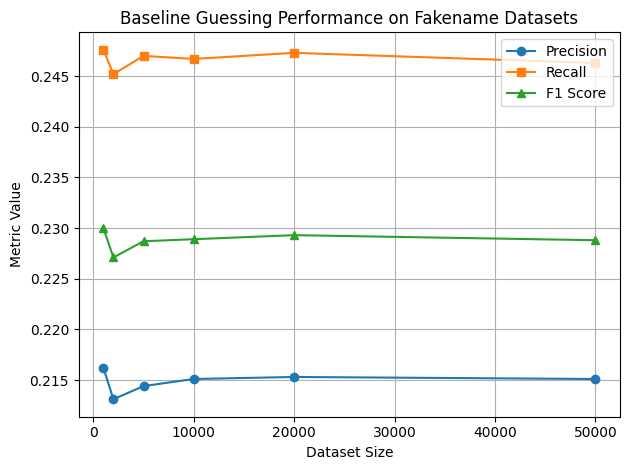
\includegraphics[width=0.5\textwidth]{img/fakename_analysis.png}
    \caption{Evaluation of the baseline performance on the \texttt{fakename} dataset: For each dataset size, the prediction quality of the 20 most frequent 2-grams is shown in terms of \textbf{precision}, \textbf{recall}, and \textbf{F1-score}. The average entry length is 21 characters.}
    \label{fig:baseline_metrics}
\end{figure}

For the \texttt{euro\_person} dataset, the baseline strategy for evaluating the effectiveness of the \ac{dea} follows the same procedure as for the \texttt{fakename} dataset.
Based on the analysis of this dataset, the average length of a full entry, comprising forename, surname, and full date of birth, is approximately 20 characters.
Assuming the use of 2-grams with overlapping character windows, this corresponds to around 19 distinct 2-grams per entry.
As a baseline, the top 19 most frequent 2-grams are selected and uniformly predicted for each record, independent of the individual characteristics of the entries.

The resulting performance metrics for this baseline prediction indicate a precision of 0.2197, a recall of 0.2446, and an F1-score of 0.2306.
These values provide an reference point for evaluating the added value of the \ac{dea} pipeline, as they quantify the effectiveness of a purely frequency driven reconstruction approach.

For the \texttt{titanic\_full} dataset, the average length of a full entry (consisting of given name and surname) is approximately 26 characters, indicating relatively high complexity due to longer names.
Therefore the top 25 most frequent 2-grams are selected as the baseline for reconstruction.
The baseline reconstruction approach achieved a precision of 0.2468, a recall of 0.3770, and an F1 score of 0.2896.
These modest performance values reflect the structural challenges posed by the dataset, including the presence of honorifics, compound names, and non-standard formatting.
The results suggest that even a naïve guessing strategy can establish a meaningful lower bound for evaluating the performance improvements of learning-based approaches such as the \ac{dea}.

Notably, for the \texttt{titanic\_full} dataset, the overlap ratio used in the experiments was adjusted to the set \{0.2, 0.4, 0.6, 0.7, 0.8, 0.9\}.
This adaptation was necessary because the dataset is relatively small, and the \ac{gma} fails to identify any individuals at lower overlap values.
Meaningful results only begin to emerge at an overlap of 0.7 or higher.

Notably, the similarity of the baseline metrics to those obtained on the \texttt{fakename} and \texttt{euro\_person} dataset highlights the generality of the method across synthetic and semi-realistic datasets, further justifying its inclusion as a comparative benchmark.

\section{Analysis}  \label{sec:analysis}

In this section the results of the \ac{dea} experiments are presented and analyzed.
The analysis is structured into several subsections, each focusing on a specific aspect of the \ac{dea} performance.
As described in Section~\ref{sec:experiments}, the experiments were conducted across multiple datasets, encoding schemes, overlaps and drop from strategies.
Therefore, several of these configuration settings will be fixed to analyze the impact of the remaining parameters on the \ac{dea} performance.

One important aspect especially for smaller datasets and overlap sizes is, that it could occur that the \ac{gma} does not identify any individuals, i.e., the re-identification set is empty.
In this case, the \ac{dea} is not able to reconstruct any plaintext information.
This is the case because if there are no re-identified individuals in place, there is no training data for the \ac{dea} available.
Therefore the results of these experiments are not reported and the corresponding data points are excluded from the analysis and plots.

The \ac{gma} could also fail during the attack by not being able to converge to a stable solution.
In this case, the \ac{dea} is not able to reconstruct any plaintext information as well.
Therefore the results of these experiments are not reported and the corresponding data points are excluded from the analysis and plots.

In total, 180 experiments were conducted to evaluate the attack's effectiveness under varying conditions, including different overlap levels and drop strategies.
On average, the \ac{dea} achieved a re-identification rate of 2.95\% and an F1-score of 0.629, with peak values reaching up to 28.75\% and 0.992, respectively.
Among the encoding schemes, \ac{tsh} exhibited the highest vulnerability with an average re-identification rate of 3.69\% and the best structural learnability (F1 = 0.688).
In contrast, \ac{tmh} yielded the lowest average re-identification rate (1.54\%) with the lowest structural learnability (F1 = 0.593), indicating greater resilience.
\ac{bf} showed a moderate performance with an average re-identification rate of 3.32\% and a structural learnability of F1 = 0.606.
The following sections analyze these results in detail, focusing on how encoding choices, dataset characteristics, and attack configurations influence the \ac{dea}'s success.


\subsection{\ac{tmh}}

The following subsection focuses on the results obtained using the \ac{tmh} encoding scheme.
In this analysis, each dataset is evaluated under varying settings.
To ensure consistency, the dataset and encoding scheme are fixed, while the evaluation focuses on the impact of different overlap sizes and drop-from strategies.

\paragraph{Titanic Full}

On the \texttt{titanic\_full} dataset, the \ac{dea} achieves stable and moderate performance using \ac{tmh} encoding.
The prediction quality improves consistently with increasing overlap between the auxiliary and target datasets (see Figure~\ref{fig:tabminhash_titanic} in Appendix~\ref{sec:tabminhash_results}).

For the \texttt{DropFrom = Eve} scenario, the F1-score decreases from 0.74 at overlap 0.7 to 0.17 at overlap 0.8, before recovering to 0.73 at overlap 0.9.
This dip at 0.8 is reflected in both recall and precision, suggesting a less effective hyperparameter configuration or reduced data utility at that particular overlap.
Precision is generally high across all overlaps, peaking at 0.96.

In the \texttt{DropFrom = Both} setting, the \ac{dea} maintains stable growth in both recall and F1-score.
Precision remains above 0.78 at all overlaps and reaches 0.96 at overlap 0.8.
At 0.9, the F1-score peaks at 0.72, confirming that even with this drop-from strategy, the \ac{dea} can learn meaningful patterns in \ac{tmh} encoded data.

Despite good predictive performance, no re-identification is achieved under any overlap or matching strategy.
Both fuzzy and greedy matching yield a re-identification rate of zero, underscoring the difficulty of exact record recovery on this small and heterogeneous dataset.



In summary, the \ac{dea} demonstrates good structural learning on \ac{tmh} encoded Titanic data, particularly at higher overlaps, but fails to produce successful record re-identifications in this configuration.


\paragraph{Fakename 1k}

On the \texttt{fakename\_1k} dataset, the \ac{dea} demonstrates moderate predictive performance when using \ac{tmh} encoding (see Figure~\ref{fig:tabminhash_fakename1k} in Appendix~\ref{sec:tabminhash_results}).
The model's ability to recover n-gram patterns improves with increasing overlap, particularly in the \texttt{DropFrom = Eve} setting.

Under \texttt{DropFrom = Eve}, F1-scores increase from 0.18 at 0.4 overlap to 0.58 at 0.8 overlap.
This trend is mainly driven by improved recall, which rises from 0.10 to 0.43, while precision remains consistently high above 0.92.
This indicates that the \ac{dea} makes accurate predictions on a small but increasing portion of the encoded data as more re-identified data becomes available.

The \texttt{DropFrom = Both} configuration shows limited performance.
Although the F1-score improves from 0.00 to 0.22 between overlaps 0.4 and 0.8, recall stays low (below 0.14), and precision only surpasses 0.85 at the highest overlap.
This suggests that the model struggles to generalize well under this drop-from strategy.

Despite some structural learning success, the re-identification rate remains at zero across all overlap values and both drop-from strategies.
Neither greedy nor fuzzy matching yields any valid mappings to original records.



Overall, the \ac{dea} on \ac{tmh} encoded \texttt{fakename\_1k} data benefits from higher overlap and the \texttt{DropFrom = Eve} strategy but remains ineffective for precise record-level re-identification.


\paragraph{Fakename 2k}

On the \texttt{fakename\_2k} dataset, the \ac{dea} shows a clear improvement in predictive performance with increasing overlap when using \ac{tmh} encoding (see Figure~\ref{fig:tabminhash_fakename2k} in Appendix~\ref{sec:tabminhash_results}).
This trend is especially evident under the \texttt{DropFrom = Eve} configuration.

In the \texttt{DropFrom = Eve} scenario, the F1-score increases from 0.10 at 0.4 overlap to 0.57 at 0.6, reaching 0.73 at 0.8.
This is driven by steady improvements in recall (from 0.06 to 0.62), while precision remains consistently high (above 0.90 at both 0.4 and 0.8).
These results suggest that the \ac{dea} learns meaningful structural patterns when sufficient re-identified training data is available.

The \texttt{DropFrom = Both} scenario shows much weaker performance.
The F1-score only reaches 0.16 at overlap 0.8, with recall staying below 0.11 and precision peaking at just 0.35.
This indicates that the \texttt{DropFrom = Both} strategy significantly limits the learning signal on smaller datasets, reducing the \ac{dea}'s effectiveness.

Re-identification remains unsuccessful across all configurations and overlaps.
Neither fuzzy nor greedy matching methods yield any valid re-identifications, which reflects the difficulty of achieving exact plaintext recovery in low-coverage scenarios.



In summary, \ac{tmh} encoding on the \texttt{fakename\_2k} dataset enables effective n-gram prediction under the \texttt{DropFrom = Eve} strategy, while re-identification remains out of reach under all tested conditions.


\paragraph{Fakename 5k}

For the \texttt{fakename\_5k} dataset, the \ac{dea} achieves strong performance in reconstructing structural patterns when \ac{tmh} is used (see Figure~\ref{fig:tabminhash_fakename5k} in Appendix~\ref{sec:tabminhash_results}).
Both \texttt{DropFrom = Eve} and \texttt{DropFrom = Both} settings show substantial improvements in predictive quality with increasing overlap.

In the \texttt{DropFrom = Eve} scenario, the F1-score rises from 0.14 at 0.2 overlap to a peak of 0.87 at 0.6.
This is supported by a corresponding increase in recall from 0.11 to 0.80, while precision exceeds 0.95 from 0.4 onward.
The \texttt{DropFrom = Both} configuration follows a similar trend, achieving an F1-score of 0.77 at 0.6 overlap, with precision of 0.98 and recall around 0.65.

Notably, this is the first setting in which the \ac{dea} yields non-zero re-identification rates.
In the \texttt{DropFrom = Eve} configuration, a re-identification rate of 1.2\% is observed at 0.6 overlap, with contributions from both fuzzy and greedy matching.
The \texttt{DropFrom = Both} setting shows a smaller but non-negligible rate of 0.07\% at the same overlap.
These results mark the transition from structural to record-level leakage under favorable training conditions.



Overall, this setting demonstrates that the \ac{dea} can become effective at re-identification as dataset size and training overlap increase.
\ac{tmh} encoded \ac{pii} becomes vulnerable to both structural inference and, under certain conditions, full record re-identification.


\paragraph{Fakename 10k}

The \ac{dea} achieves high performance on the \texttt{fakename\_10k} dataset with \ac{tmh} encoding (see Figure~\ref{fig:tabminhash_fakename10k} in Appendix~\ref{sec:tabminhash_results}).
Both predictive quality and re-identification effectiveness increase significantly with overlap, particularly under the \texttt{DropFrom = Eve} scenario.

In the \texttt{DropFrom = Eve} scenario, the F1-score improves from 0.51 at 0.2 overlap to 0.93 at 0.6 and 0.92 at 0.8.
Precision remains consistently above 0.96, and recall exceeds 0.9 at the two highest overlaps.
The model clearly benefits from access to a larger fraction of re-identified training data, leading to near-perfect structural reconstruction.

The \texttt{DropFrom = Both} configuration follows a similar trend but with slightly lower performance at small overlaps.
At 0.8 overlap, it reaches an F1-score of 0.91, with precision of 0.98 and recall of 0.86.
Compared to smaller datasets, performance differences between the two dropout strategies become marginal at high overlaps.

For the first time, substantial re-identification rates are observed.
Under \texttt{DropFrom = Eve}, the combined re-identification rate reaches 5.45\% at 0.6 overlap and remains above 5\% at 0.8.
The \texttt{DropFrom = Both} configuration achieves a lower peak of 2.97\% at 0.8.
Both fuzzy and greedy methods contribute to these results, with fuzzy matching consistently recovering more records.

These findings are mirrored in the aggregate relationship between F1-score and re-identification rate, which shows a clear positive correlation. This confirms that structural accuracy translates to successful record-level attacks in larger datasets.



Overall, the \ac{dea} is highly effective on \ac{tmh} encoded data when training coverage is sufficient and dataset size enables generalization.
The combination of high recall and precision leads to significant re-identification risk at overlap levels of 0.6 and above.


\paragraph{Fakename 20k}

The \ac{dea} reaches its highest level of effectiveness on the \texttt{fakename\_20k} dataset when using \ac{tmh} encoding (see Figure~\ref{fig:tabminhash_fakename20k} in Appendix~\ref{sec:tabminhash_results}).
Both structural reconstruction and re-identification performance scale with dataset size and overlap, confirming the vulnerability of \ac{tmh} encoded data under \ac{dea}s.

In the \texttt{DropFrom = Eve} configuration, F1-scores increase from 0.51 at 0.2 overlap to 0.96 at 0.8.
Precision and recall both exceed 0.95 at the highest overlap, indicating that the model is able to reconstruct the n-gram distribution with high fidelity.
The \texttt{DropFrom = Both} setting follows a similar trajectory, with the F1-score reaching 0.95 at 0.8 and precision nearly identical to the Eve scenario.

The re-identification rates increase sharply with overlap.
Under \texttt{DropFrom = Eve}, the combined re-identification rate reaches 13.47\% at 0.8, with greedy and fuzzy matching each contributing a substantial portion.
Even in the more conservative \texttt{DropFrom = Both} setting, the rate surpasses 10\% at the highest overlap, confirming that re-identification is possible even without access to a clean subset.

The correlation between F1-score and re-identification rate is stronger than in previous datasets, with a visibly steep upward trend.
This suggests that small improvements in structural accuracy have increasingly large effects on re-identification success in large-scale datasets.



In summary, the \texttt{fakename\_20k} experiments demonstrate the full potential of the \ac{dea}.
With high overlap and sufficient data, \ac{tmh} encoding fails to protect against meaningful reconstruction and record-level compromise.


\paragraph{Europerson}

The \textit{euro person} dataset further confirms the vulnerability of \ac{tmh} encodings under \ac{dea}s (see Figure~\ref{fig:tabminhash_euro} in Appendix~\ref{sec:tabminhash_results}).
Despite variations in overlap, the \ac{dea} consistently achieves high predictive performance and exhibits meaningful re-identification capability.

Across all overlap values, the model maintains high precision (above 0.92), with only moderate variability in recall.
In the \texttt{DropFrom = Both} setting, F1-scores exceed 0.87 at all overlaps and peak at 0.94 for overlap 0.4.
The \texttt{DropFrom = Eve} configuration shows more fluctuation, with F1-scores ranging from 0.50 to 0.92, likely due to reduced training set size at lower overlaps.

Re-identification rates vary substantially across overlaps.
In the \texttt{DropFrom = Both} setting, a peak re-identification rate of 6.85\% is observed at overlap 0.6.
Notably, this rate drops to near zero at 0.8, despite similar predictive metrics, indicating the effect of reduced unique reconstruction under high training similarity.
The \texttt{DropFrom = Eve} setting shows similar behavior with a maximum re-identification rate of 6.12\% at 0.6 overlap, largely driven by greedy matches.

The aggregate F1-to-re-identification relationship exhibits a clear positive trend, reinforcing that high structural accuracy translates into privacy loss at the record level.
This is further supported by the distribution of fuzzy and greedy re-identifications, with both contributing significantly at intermediate overlaps.



Overall, the \textit{euro person} dataset reveals that even realistic data encoded via \ac{tmh} is susceptible to reconstruction and re-identification.
The \ac{dea} performs reliably across settings, with overlap 0.6 appearing to maximize re-identification success.


\paragraph{Summary Across Datasets and Overlap Levels}

Figure~\ref{fig:tabminhash_overlap} in Appendix~\ref{sec:tabminhash_results} illustrates the relationship between overlap and both re-identification rate (left) and F1-score (right), averaged over drop strategies for each dataset.
The results highlight how both structural and record-level vulnerabilities evolve with dataset size and training coverage.

Larger datasets such as \texttt{fakename\_20k}, \texttt{fakename\_10k}, and \texttt{euro\_person} exhibit clear monotonic trends.
As the overlap increases, both F1-scores and re-identification rates improve.
For \texttt{fakename\_20k}, the re-identification rate peaks at nearly 12\% for 0.8 overlap.
Similarly, \texttt{euro\_person} reaches its highest F1-score at 0.6 overlap, accompanied by its highest re-identification performance, indicating that structural accuracy enables effective exploitation.

Smaller datasets such as \texttt{fakename\_1k}, \texttt{fakename\_2k}, and \texttt{titanic\_full} show limited gains in re-identification, regardless of overlap.
Their F1-scores increase with overlap, but remain insufficient to enable consistent reconstruction.
Notably, \texttt{fakename\_5k} serves as a transition point: at 0.6 overlap, it achieves a modest re-identification rate and solid F1-score, but both metrics drop again at 0.8 overlap.

Across datasets, the plots reveal that higher overlap generally yields better F1-scores.
However, effective re-identification is highly dependent on dataset size and complexity.
The correlation between these two metrics is dataset-specific and non-linear, particularly at high F1 values where small increases may lead to steep jumps in re-identification.

These findings reinforce the conclusion that \ac{tmh} encodings do not provide sufficient protection in high-overlap, large-scale scenarios.
While the \ac{dea} may remain ineffective on small or disjoint datasets, it becomes increasingly potent as structural learning converges, ultimately compromising encoded identifiers.

\paragraph{Architecture}

Figure~\ref{fig:tabminhash_architecture} in Appendix~\ref{sec:tabminhash_results} presents a distributional analysis of the neural network architectures selected during hyperparameter optimization across all \ac{tmh} experiments.
The results provide insight into which architectural choices consistently yield strong performance in structural reconstruction and re-identification tasks.

The majority of optimized models employ a shallow architecture with a single hidden layer.
More complex configurations with two or three layers are rare, suggesting that the \ac{dea} can learn effective representations without requiring deep hierarchical abstraction.
This is consistent with the relatively structured nature of the prediction task and the compactness of \ac{tmh} encoded records.

In terms of hidden size, larger configurations are clearly favored.
The most frequent choice is a hidden dimension of 2048, followed by 1024.
Smaller sizes below 512 occur infrequently, indicating that wide layers contribute significantly to capturing the necessary n-gram co-occurrence patterns for decoding.

Dropout rates are broadly distributed, with a mean around 0.24.
This suggests that regularization is helpful, but not critical; overfitting appears to be limited even with lower dropout.
The threshold histogram indicates that models typically settle around a value of 0.44 for binary classification, though a wide range is explored, reflecting dataset-specific optimality.

Activation functions are led by \texttt{elu} and \texttt{selu}, both of which support smooth non-linear transitions and internal normalization.
Simpler functions like \texttt{relu} and \texttt{gelu} are used less frequently.
This preference for normalized activations may reflect the benefits of stability during training on small gradients.

Among optimizers, \texttt{AdamW} is most commonly selected, followed by \texttt{Adam} and \texttt{\texttt{RMSprop}}.
This aligns with the need for stable adaptive learning rates and effective weight decay.
Learning rate schedulers are also diverse, with \texttt{ReduceLROnPlateau} and \texttt{CyclicLR} being the most frequent.
The inclusion of schedulers reflects their utility in adjusting learning dynamics over the short training windows.

Batch sizes of 8 and 16 dominate, likely due to the small to medium dataset sizes.
Finally, the number of training epochs converges to 20 in nearly all cases, the maximum allowed during tuning, suggesting that performance continues to improve up to the epoch limit.

In summary, the optimal architecture for \ac{tmh} encoded \ac{dea} models is characterized by a shallow but wide feedforward network, mild regularization, normalized activations, and adaptive optimizers with scheduler support.
These configurations are robust across datasets and contribute significantly to the attack's effectiveness.

\subsection{\ac{tsh}}

The following subsection focuses on the results obtained using the \ac{tsh} encoding scheme.
In this analysis, each dataset is evaluated under varying settings.
To ensure consistency, the dataset and encoding scheme are fixed, while the evaluation focuses on the impact of different overlap sizes and drop-from strategies.

\paragraph{Titanic Full}

On the \texttt{titanic\_full} dataset, the \ac{dea} performs reliably when using \ac{tsh} encoding, achieving stable precision and recall across overlap values (see Figure~\ref{fig:twostep_titanic} in Appendix~\ref{sec:twostep_results}).
F1-scores range from 0.34 to 0.83, depending on the drop strategy and overlap.

In the \texttt{DropFrom = Eve} setting, the model consistently achieves high precision (above 0.95) across all tested overlaps.
Recall improves with overlap, rising from 0.56 at 0.7 to 0.74 at 0.9.
The resulting F1-score increases accordingly, reaching a maximum of 0.83 at 0.9 overlap, indicating robust learning from partially re-identified data even in small datasets.

The \texttt{DropFrom = Both} configuration shows more variability.
At 0.7 overlap, the F1-score remains low at 0.34, reflecting low precision (0.26) despite moderate recall (0.55).
However, at 0.8 overlap, both precision and recall improve, yielding an F1-score of 0.72.
This suggests that the \texttt{DropFrom = Both} strategy can be mitigated as overlap increases, but model reliability depends strongly on sample size.

No re-identifications are observed at any overlap level for either drop-from strategy.
Both fuzzy and greedy matching yield zero hits, highlighting that accurate structural predictions do not necessarily lead to successful record reconstruction in small datasets like \texttt{titanic\_full}.



In summary, \ac{tsh} provides solid predictive performance on the \texttt{titanic\_full} dataset, particularly when Eve's overlap is high.
Nonetheless, the attack remains structurally bounded, and record-level re-identification is not achieved.


\paragraph{Fakename 1k}

On the \texttt{fakename\_1k} dataset, the \ac{dea} shows measurable improvements in structural prediction performance as the overlap increases, though it fails to achieve any successful re-identifications (see Figure~\ref{fig:twostep_fakename1k} in Appendix~\ref{sec:twostep_results}).

In the \texttt{DropFrom = Eve} setting, F1-scores rise sharply with overlap, starting from 0.11 at 0.4 to 0.74 at 0.8.
This trend is driven by improvements in both recall (from 0.06 to 0.62) and precision (from 0.52 to 0.95).
The results suggest that the \ac{dea} is able to learn useful representations even with a small dataset, provided sufficient re-identified training data is available.

The \texttt{DropFrom = Both} configuration performs worse, particularly at lower overlaps.
At 0.6 overlap, F1-score remains low (0.07), but rises to 0.66 at 0.8, supported by high precision (0.95) and moderate recall (0.52).

Despite achieving F1-scores over 0.7 in some configurations, re-identification remains at 0\% for all tested overlaps and matching strategies.
This underlines the fact that a strong n-gram prediction model does not necessarily translate into record-level success when the dataset size is small.



Overall, \ac{tsh} yields competitive structural predictions on small datasets like \texttt{fakename\_1k}, particularly when the training overlap is high.
However, the \ac{dea} does not succeed in reconstructing any individual records in this configuration.



\paragraph{Fakename 2k}

The \texttt{fakename\_2k} dataset reveals a clear improvement in \ac{dea} performance with increasing overlap when \ac{tsh} encoding is used (see Figure~\ref{fig:twostep_fakename2k} in Appendix~\ref{sec:twostep_results}).
While low-overlap configurations perform poorly, both structural prediction and re-identification become feasible at higher overlaps.

In the \texttt{DropFrom = Eve} setting, the F1-score increases from 0.11 at 0.2 to 0.76 at 0.6, and further to 0.83 at 0.8.
Precision remains high throughout (above 0.79), while recall improves substantially with overlap.
These results indicate that once a sufficient number of re-identified records are available, the \ac{dea} can learn and generalize the underlying encoding structure effectively.

The \texttt{DropFrom = Both} configuration follows a similar trend but lags slightly.
At 0.4 overlap, performance remains negligible (F1 = 0.11), but at 0.8 it rises to 0.83, with both precision (0.97) and recall (0.74) being strong.
This confirms that the \texttt{DropFrom = Both} strategy can be overcome given sufficient overlap.

Unlike on the 1k dataset, the \ac{dea} successfully re-identifies individual records at higher overlaps. Under \texttt{DropFrom = Eve}, a small re-identification rate of 0.1\% is achieved at 0.6.
In the \texttt{DropFrom = Both} setting, this increases to 0.3\% at 0.8.
Although the rates are modest, they demonstrate that re-identification becomes possible as structural accuracy increases.

The trend between F1-score and re-identification rate is consistent, with successful re-identifications only occurring beyond F1 = 0.75.
This reflects a threshold-like behavior in the attack's effectiveness.



In summary, the \texttt{fakename\_2k} dataset shows that \ac{tsh} encoding provides limited protection once the overlap exceeds 0.6.
The \ac{dea} can achieve strong predictions and initial re-identifications even in modestly sized datasets.


\paragraph{Fakename 5k}

The \texttt{fakename\_5k} dataset marks the transition point where the \ac{dea} begins to yield meaningful re-identification rates under \ac{tsh} encoding (see Figure~\ref{fig:twostep_fakename5k} in Appendix~\ref{sec:twostep_results}).
Both precision and recall improve steadily with increasing overlap, and re-identification becomes feasible.

In the \texttt{DropFrom = Eve} setting, the model achieves an F1-score of 0.10 at 0.2 overlap, but quickly improves to 0.89 at 0.6, with near-perfect precision (0.99) and strong recall (0.82).
Interestingly, performance slightly drops at 0.8, suggesting that the increased overlap does not always translate to higher generalization capacity under this drop strategy.

The \texttt{DropFrom = Both} configuration follows a smoother trajectory.
F1-score increases from 0.22 at 0.2 overlap to 0.76 at 0.4, 0.89 at 0.6, and peaks at 0.94 at 0.8.
These results are underpinned by consistently high precision and rising recall, indicating the model's ability to capture \ac{tmh} encoded structure even under the \texttt{DropFrom = Both} strategy.

The first substantial re-identification rates are observed in this dataset.
Under \texttt{DropFrom = Eve}, the combined rate reaches 2.1\% at 0.6 but drops again at 0.8.
In contrast, \texttt{DropFrom = Both} shows increasing re-identification, reaching 5.52\% at 0.8.

The re-identification curve as a function of F1-score shows the expected upward trend, confirming that strong structural prediction is a prerequisite for record-level re-identification.



Overall, the \texttt{fakename\_5k} dataset demonstrates that \ac{dea} success under \ac{tsh} encoding is strongly dependent on overlap and dataset size.
Once a critical threshold is reached, even structurally obfuscated data becomes vulnerable to reconstruction.



\paragraph{Fakename 10k}

The \ac{dea} achieves consistently high structural prediction performance on the \texttt{fakename\_10k} dataset when using \ac{tsh} encoding (see Figure~\ref{fig:twostep_fakename10k} in Appendix~\ref{sec:twostep_results}).
Re-identification becomes substantial, particularly in the \texttt{DropFrom = Eve} configuration at intermediate overlaps.

In the \texttt{DropFrom = Eve} scenario, F1-scores are strong across all overlaps: 0.87 at 0.2, rising to 0.94 at 0.6, before slightly decreasing to 0.75 at 0.8.
These fluctuations are primarily driven by changes in recall, which peaks at 0.90 but drops sharply at 0.8, despite stable precision above 0.96 throughout.
This indicates that excessive overlap may not always improve performance due to overfitting or reduced variance in the training set.

The \texttt{DropFrom = Both} configuration shows more stability at high overlaps.
F1-scores increase from 0.76 at 0.2 to 0.91 at 0.4, and finally 0.94 at 0.8.
At 0.6, however, the model fails to generalize, with recall collapsing to 0.05 and F1 dropping to 0.10.
This suggests a sensitivity to training set composition at this overlap.

Re-identification rates are highest for Eve at 0.6 overlap (10.9\%), coinciding with its peak in F1-score.
The \texttt{DropFrom = Both} setup reaches a maximum re-identification rate of 5.6\% at 0.8.
Fuzzy and greedy matching contribute similarly to the results, with combined predictions amplifying the attack's effectiveness.

The re-identification rate shows a non-linear but positively correlated relationship with F1-score.
The strongest privacy breaches occur in the range F1 > 0.9, highlighting the tipping point at which structural reconstruction translates into record-level re-identification.

In summary, the fakename 10k dataset confirms that \ac{dea} success under \ac{tsh} encoding scales with dataset size and overlap.
However, unexpected performance drops can occur under certain conditions, emphasizing the need for robust model selection.


\paragraph{Fakename 20k}

The \texttt{fakename\_20k} dataset confirms the scalability and effectiveness of the \ac{dea} when applied to large, \ac{tsh} encoded datasets (see Figure~\ref{fig:twostep_fakename20k} in Appendix~\ref{sec:twostep_results}).

In the \texttt{DropFrom = Eve} configuration, the \ac{dea} achieves F1-scores of 0.94, 0.97, and 0.99 at overlaps 0.2, 0.4, and 0.8, respectively.
Both precision and recall are near 1.0 throughout, indicating highly reliable reconstruction of the encoded representations.
In the \texttt{DropFrom = Both} case, the model achieves an F1-score of 0.92 at 0.8 overlap with a precision of 0.99 and recall of 0.86, again showing strong generalization under \texttt{DropFrom = Both}.

Under \texttt{DropFrom = Eve}, the rate increases from 5.73\% at 0.2 overlap to 13.20\% at 0.4, and further to 23.00\% at 0.8.
The combined matching strategy benefits from contributions by both fuzzy and greedy methods, peaking at over 23\%.

In the \texttt{DropFrom = Both} setting, the re-identification rate reaches 2.49\% at 0.8 overlap.
While lower than in the \texttt{DropFrom = Eve} case, this still represents a notable privacy breach.

The positive linear trend between F1-score and re-identification rate is especially clear in this dataset, with a nearly perfect fit across configurations.
This reinforces the conclusion that once structural accuracy exceeds 0.9, re-identification becomes a likely outcome.

In summary, the \texttt{fakename\_20k} experiments demonstrate high vulnerability of \ac{tsh} encoded databases under \ac{dea}s.
Even with minimal overlap, the \ac{dea} can achieve both high reconstruction fidelity and impactful re-identification, posing a serious threat to encoded privacy-preserving record linkage.


\paragraph{Europerson}

The \texttt{euro\_person} dataset yields the highest observed re-identification rates under \ac{tsh} encoding.
Structural prediction performance is nearly perfect across all overlap values, and re-identification success exceeds 20\% at high overlap.

In the \texttt{DropFrom = Eve} configuration, the model achieves F1-scores above 0.98 for overlaps 0.6 and 0.8.
Precision and recall are both near 1.0, indicating that the model captures the encoded structure with high fidelity.
Even at 0.2 overlap, the F1-score remains strong at 0.93, supported by a recall of 0.90 and precision of 0.95.

The \texttt{DropFrom = Both} setting shows similar behavior.
The F1-score rises from 0.68 at 0.2 to 0.98 at 0.6 and 0.99 at 0.8.
This suggests that sufficient overlap renders the \ac{dea} robust even under this drop-from strategy.

Re-identification rates are particularly striking.
Under \texttt{DropFrom = Eve}, the combined matching method reaches 22.6\% at 0.6 overlap and remains stable at 22.3\% at 0.8.
The corresponding values in the \texttt{DropFrom = Both} setting are 17.8\% and 21.9\%, respectively.

The re-identification curve versus F1-score shows a near-linear relationship with a steep slope, underscoring the strong coupling between model accuracy and privacy leakage.

In summary, the \texttt{euro\_person} dataset illustrates that the combination of \ac{tsh} encoding and realistic, high-quality input data is particularly vulnerable to \ac{dea}s.
The \ac{dea} can achieve both high prediction fidelity and extensive re-identification success, even with limited initial overlap.

\paragraph{Summary Across Datasets and Overlap Levels}

The summary plots in Figure~\ref{fig:twostep_overlap} in Appendix~\ref{sec:twostep_results} illustrate the overall relationship between overlap, structural prediction quality, and re-identification success across all evaluated datasets using \ac{tsh} encoding.

Across all datasets, F1-scores generally increase with overlap, reflecting improved structural learning by the neural model as more training data becomes available.
For small datasets like \texttt{titanic\_full} and \texttt{fakename\_1k}, the \ac{dea} struggles until the overlap reaches 0.8.
In contrast, medium-sized datasets such as \texttt{fakename\_5k} and \texttt{fakename\_10k} show steep improvements between 0.4 and 0.6.
Larger datasets (\texttt{fakename\_20k} and \texttt{euro\_person}) achieve F1-scores above 0.9 even at lower overlaps (0.2 or 0.4), confirming their higher learnability.

Re-identification success remains low in small datasets, regardless of F1-score.
In \texttt{fakename\_1k}, \texttt{fakename\_2k}, and \texttt{titanic\_full}, the \ac{dea} fails to re-identify any records.
The first meaningful re-identification rates emerge in \texttt{fakename\_5k}, reaching up to 2.5\% at 0.8 overlap.
In \texttt{fakename\_10k}, the rate peaks at 5.8\% at overlap 0.6 but decreases slightly at 0.8.
\texttt{fakename\_20k} shows relatively stable re-identification performance across overlaps, with rates of 5.7\%, 13.2\%, and 12.8\% at overlaps 0.2, 0.4, and 0.8, respectively.
The \texttt{euro\_person} dataset is the most vulnerable, with a re-identification rate of 20.4\% at 0.6 and peaking at 22.9\% at 0.8.

These results confirm a non-linear but consistent dependency between structural performance and re-identification capability.
Notably, some datasets exhibit diminishing returns at very high overlaps, potentially due to reduced variability or model overfitting.
Additionally, privacy leakage appears to depend not only on model performance (F1) but also on dataset characteristics such as name structure, token diversity, and size.

Overall, \ac{tsh} poses a clear privacy risk under \ac{dea}s.
While encoding obfuscates raw values, neural networks trained on auxiliary data can learn the structural mapping and enable re-identification—especially in realistic, large-scale datasets.


\paragraph{Architecture}

Figure~\ref{fig:twostep_architecture} in Appendix~\ref{sec:twostep_results} shows the distributions of the best-performing neural network configurations for models trained on \ac{tsh} encoded datasets.
Most models are relatively shallow: the majority use a single hidden layer, indicating that deeper networks are not necessary to capture the structure of the encoding.
At the same time, the preferred hidden size is large, with 2048 being the most frequent choice, suggesting that a wide representation is crucial for learning the mapping from encoded inputs to class labels.

In terms of activation functions, \texttt{gelu} and \texttt{selu} are most often selected, while traditional choices like \texttt{relu}, \texttt{tanh}, and \texttt{leaky\_relu} appear less frequently.
This preference points to the importance of smooth and differentiable non-linearities that preserve gradient flow.
Optimizer selection favors \texttt{RMSprop}, followed by Adam and AdamW.
\texttt{RMSprop}'s popularity may be due to its ability to handle sparse and noisy gradients effectively.
Learning rate schedulers are used in most cases, with \texttt{None} and \texttt{CyclicLR} dominating.
This reflects that both fixed and adaptive schedules can work well depending on dataset size and overlap.

Regularization is handled via dropout, with most selected values ranging between 0.15 and 0.35 (mean: 0.25), indicating a moderate level of regularization is helpful to avoid overfitting to the structure of the extended training data.
The decision threshold for classification tends to cluster around 0.39.
Most models train for around 15–20 epochs, with a noticeable concentration at the upper bound, suggesting that full training cycles are often required to reach convergence.
Small batch sizes, particularly 8 and 16, dominate, likely due to their regularizing effect and suitability for noisy structural input.

\subsection{\ac{bf}}

The following subsection focuses on the results obtained using the \ac{bf} encoding scheme.
In this analysis, each dataset is evaluated under varying settings.
To ensure consistency, the dataset and encoding scheme are fixed, while the evaluation focuses on the impact of different overlap sizes and drop-from strategies.

\paragraph{Titanic Full}

On the \texttt{titanic\_full} dataset, the \ac{dea} demonstrates strong structural learning capabilities when using \ac{bf} encoding (see Figure~\ref{fig:bloomfilter_titanic} in Appendix~\ref{sec:bloomfilter_results}).

At overlap 0.9, the model reaches an F1-score of 0.83 under the \texttt{DropFrom = Eve} strategy, indicating that the structural mapping between encoded and raw data can be learned to a high degree.
With the \texttt{DropFrom = Both} strategy, the model performs slightly worse with an F1-score of 0.81.
While the precision is consistently high in both cases (above 0.95), recall increases significantly with higher overlap and is consistently better when training on \texttt{DropFrom = Eve}.

Despite strong structural performance, no successful re-identifications were made, regardless of overlap or re-identification strategy.
Both fuzzy and greedy matching yield zero hits, highlighting that accurate structural predictions do not necessarily lead to successful record reconstruction in small datasets like \texttt{titanic\_full}.

In summary, \ac{bf} provides solid predictive performance on the \texttt{titanic\_full} dataset, particularly when \texttt{DropFrom = Eve} is used.
Nonetheless, the attack remains structurally bounded, and record-level re-identification is not achieved.

\paragraph{Fakename 1k}

On the \texttt{fakename\_1k} dataset, the \ac{dea} shows moderate performance when using \ac{bf} encoding (see Figure~\ref{fig:bloomfilter_fakename1k} in Appendix~\ref{sec:bloomfilter_results}).
Performance varies notably depending on the drop strategy.

Under the \texttt{DropFrom = Eve} setting, the model achieves a peak F1-score of 0.67 at overlap 0.8.
Precision reaches over 0.9, while recall follows a similar trend, confirming that overlap and drop strategy significantly influence learnability.

The \texttt{DropFrom = Both} configuration shows consistently lower performance, with F1-scores never exceeding 0.20.
Precision remains low for this strategy, indicating that the model struggles to generalize well under this drop-from strategy.

Despite the difference in structural performance, no re-identifications are made at any overlap or with any matching method.
As before, the attack manages to recover structural patterns when training data is suitable, but \ac{bf}s at this scale appear to prevent any meaningful semantic reconstruction.

Overall, \ac{bf} yields competitive structural predictions on small datasets like \texttt{fakename\_1k}, particularly when the training overlap is high.
However, the \ac{dea} does not succeed in reconstructing any individual records in this configuration.

\paragraph{Fakename 2k}

For the \texttt{fakename\_2k} dataset, the \ac{dea} shows clear improvement in predictive performance with increasing overlap when \ac{bf} encoding is used (see Figure~\ref{fig:bloomfilter_fakename2k} in Appendix~\ref{sec:bloomfilter_results}).

Under the \texttt{DropFrom = Eve} setting, the attack reaches an F1-score of 0.86 at overlap 0.8.
This is supported by both precision and recall exceeding 0.8, indicating robust learning from partially re-identified data.

The \texttt{DropFrom = Both} configuration shows weaker performance, yielding an F1-score of 0.72 at the same overlap.
This discrepancy mirrors the gap in recall and precision between the two conditions, with recall remaining below 0.7 for the \texttt{DropFrom = Both} strategy.

Unlike previous datasets, \ac{bf} encoding begins to show measurable vulnerability.
The re-identification rate reaches 1.5\% in the best case (overlap 0.8, \texttt{DropFrom = Eve}), with most successful re-identifications resulting from the fuzzy matching strategy.

The comparison between F1-score and re-identification rate shows a clear positive correlation, confirming that structural accuracy translates to successful record-level attacks.

In summary, the \texttt{fakename\_2k} dataset shows that \ac{bf} encoding provides limited protection once the overlap exceeds 0.8.
The \ac{dea} can achieve strong predictions and initial re-identifications even in modestly sized datasets.

\paragraph{Fakename 5k}

The \texttt{fakename\_5k} dataset exhibits a noticeable rise in vulnerability under \ac{bf} encoding (see Figure~\ref{fig:bloomfilter_fakename5k} in Appendix~\ref{sec:bloomfilter_results}).

At overlap 0.6, the model trained on \texttt{DropFrom = Eve}  achieves an F1-score of 0.93, clearly surpassing the performance of the model trained with the \texttt{DropFrom = Both} strategy (F1 = 0.90).
For overlap 0.8, the scores diverge more strongly: the F1-score drops to 0.49 for \texttt{DropFrom = Eve}, while it remains high at 0.87 for \texttt{DropFrom = Both}.
This inversion suggests a shift in learning dynamics where a larger overlap allows the model trained on \texttt{DropFrom = Both} to generalize better, possibly due to higher variance in the training set.

The re-identification rate peaks at overlap 0.6, with 5.1\% when trained on \texttt{DropFrom = Eve} and 1.6\% for \texttt{DropFrom = Both}.

Compared to \texttt{fakename\_2k}, the attacker gains more leverage here.
While the F1-score improves only slightly, the re-identification rate scales more than threefold, indicating that higher dataset contributes to exploitability.

The re-identification curve as a function of F1-score shows the expected upward trend, confirming that strong structural prediction is a prerequisite for record-level re-identification.

Overall, the \texttt{fakename\_5k} dataset demonstrates that \ac{dea} success under \ac{bf} encoding is strongly dependent on overlap and dataset size.
Once a critical threshold is reached, even structurally obfuscated data becomes vulnerable to reconstruction.

\paragraph{Fakename 10k}

The results on \texttt{fakename\_10k} mark a transition where the dataset size and model capacity jointly enable highly effective re-identification under \ac{bf} encoding (see Figure~\ref{fig:bloomfilter_fakename10k} in Appendix~\ref{sec:bloomfilter_results}).

The F1-score reaches a peak of 0.95 for \texttt{DropFrom = Eve} and 0.94 for \texttt{DropFrom = Both} at overlap 0.6.
For both drop-from strategies, this overlap corresponds to the best-performing configuration.
At overlap 0.8, both models maintain high performance, although \texttt{DropFrom = Both} starts to degrade more steeply (F1 = 0.81 vs. 0.88 for \texttt{DropFrom = Eve}).

Re-identification is most successful at overlap 0.6, with rates of 11.1\% and 7.9\% for \texttt{DropFrom = Eve} and \texttt{DropFrom = Both}, respectively.
As before, the greedy matchins strategy yields the best results.

The fitted curve shows a positive relation between F1 and re-identification rate, confirming that performance gains increasingly translate to effective attacks beyond a certain threshold.

In summary, the \texttt{fakename\_10k} dataset confirms that \ac{dea} success under \ac{bf} encoding scales with dataset size and overlap.
However, unexpected performance drops can occur under certain dropout conditions, emphasizing the need for robust model selection.

\paragraph{Fakename 20k}

The \texttt{fakename\_20k} dataset yields high re-identification rates under \ac{bf} encoding (see Figure~\ref{fig:bloomfilter_fakename20k} in Appendix~\ref{sec:bloomfilter_results}).

At overlap 0.8, the trained model achieves F1-scores of 0.97 and 0.96 for \texttt{DropFrom = Eve} and \texttt{DropFrom = Both}, respectively.
These near-perfect values are accompanied by precision values above 0.99 and recall values exceeding 0.93.
The overall performance of the neural network remains stable across the entire overlap range, starting already at an F1-score of 0.83 for the lowest evaluated overlap of 0.2 (\texttt{DropFrom = Eve}).

Re-identification rates increase monotonically with overlap.
At overlap 0.8, \texttt{DropFrom = Eve} yields a re-identification rate of 19.2\%.
\texttt{DropFrom = Both} yields a lower rate of 11.1\%, but even this value is poses a serious threat.
Decomposing the re-identification results reveals that the greedy method dominates.

The positive linear trend between F1-score and re-identification rate is especially clear in this dataset, with a nearly perfect fit across configurations.
This reinforces the conclusion that once structural accuracy exceeds 0.9, re-identification becomes a likely outcome.

In summary, the \texttt{fakename\_20k} experiments demonstrate high vulnerability of \ac{bf} encoded databases under \ac{dea}s.
Even with minimal overlap, the \ac{dea} can achieve both high reconstruction fidelity and impactful re-identification, posing a serious threat to encoded privacy-preserving record linkage.

\paragraph{Euro Person}

The \texttt{euro\_person} dataset yields the highest observed re-identification rates under \ac{bf} encoding (see Figure~\ref{fig:bloomfilter_europerson} in Appendix~\ref{sec:bloomfilter_results}).

Due to computational limitations encountered during the \ac{gma} phase, results are only available for overlap 0.8.
The \ac{gma} failed to converge at lower overlap levels (0.2, 0.4, 0.6) due to the presence of non-finite values in the similarity matrix, which caused the singular value decomposition algorithm to encounter numerical instabilities.
This limitation reflects the computational challenges associated with large-scale similarity computations in high-dimensional encoding spaces.

At overlap 0.8, the trained model achieves F1-scores of 0.9915 and 0.9886 for \texttt{DropFrom = Eve} and \texttt{DropFrom = Both}, respectively.
These values are accompanied by near-perfect precision (0.9946 and 0.9961) and recall (0.9890 and 0.9819), underscoring the \ac{dea}'s capacity to learn the structural patterns of \ac{bf} encodings with high fidelity.

Re-identification rates reflect this structural success.
\texttt{DropFrom = Eve} yields a re-identification rate of 28.75\%, the highest recorded in the evaluation.
\texttt{DropFrom = Both} results in a slightly lower but still critical rate of 20.77\%.
These results confirm that \ac{bf} encodings of semi-realistic identifiers become highly vulnerable to inference once a sufficient portion of the dataset is re-identified.

In summary, the \texttt{euro\_person} experiments illustrate that \ac{bf} encodings fail to provide adequate protection under \ac{dea}s in high-overlap, high-structure scenarios.
The attack achieves both high predictive performance and substantial re-identification rates, confirming the practical threat to encoded privacy-preserving record linkage in real-world settings.


\paragraph{Summary Across Datasets and Overlap Levels}

Figure~\ref{fig:bloomfilter_overlap} in Appendix~\ref{sec:bloomfilter_results} illustrates the relationship between overlap and both re-identification rate (left) and F1-score (right), averaged over drop strategies for each dataset.
The results highlight how both structural and record-level vulnerabilities evolve with dataset size and training coverage.

The overall performance of the \ac{dea} with \ac{bf} encodings shows clear dependencies on both dataset size and overlap.
Larger datasets enable significantly higher re-identification rates and F1-scores.
On the \texttt{fakename\_20k} dataset, re-identification peaks at 17.6\% at an overlap of 0.6, while the F1-score consistently exceeds 0.95 across all overlap levels.
Similarly, the \texttt{euro\_person} dataset shows the highest observed re-identification rate of 28.75\% at overlap 0.8, with a corresponding F1-score of 0.99.

In contrast, datasets with fewer than 5{,}000 entities yield only minimal re-identifications, even when model performance is moderately high.
For instance, \texttt{fakename\_2k} and \texttt{fakename\_1k} exhibit low re-identification rates (below 1.5\%), despite achieving F1-scores around 0.79 and 0.44, respectively, at high overlap.
On \texttt{titanic\_full}, the \ac{dea} achieves modest F1-scores near 0.43 but fails to re-identify any records.

A general trend is observable: for all datasets, F1-score improves with increasing overlap.
However, re-identification rates do not scale linearly with model performance.
Some configurations (e.g., \texttt{fakename\_10k} and \texttt{fakename\_20k}) exhibit a peak at intermediate overlaps (e.g., 0.6), suggesting a trade-off between memorization and generalization during training.
In these cases, higher overlap may reduce variance in the training set and unintentionally impair generalization.

These findings confirm that \ac{bf}s remain a robust encoding for small-scale linkage scenarios but fail to offer sufficient protection in larger datasets under realistic threat models.
The \ac{dea} becomes increasingly effective with scale and overlap, particularly in the presence of sufficient training data and favorable \ac{gma} conditions.


\paragraph{Architecture}

Figure~\ref{fig:bloomfilter_architecture} in Appendix~\ref{sec:bloomfilter_results} presents a distributional analysis of the neural network architectures selected during hyperparameter optimization across all \ac{bf} experiments.
The results provide insight into which architectural choices consistently yield strong performance in structural reconstruction and re-identification tasks.

The architectural configurations chosen during hyperparameter optimization for \ac{bf} encodings reveal a strong preference for compact, shallow networks.
The majority of trained models used a single hidden layer, combined with a hidden size of 2048 neurons.
Smaller hidden sizes were rarely selected.

Dropout rates clustered around 0.27 on average, with moderate variance, suggesting that regularization was important to avoid overfitting.
Threshold values after sigmoid activation centered around 0.39, reflecting the relatively conservative decision boundaries necessary when working with noisy encodings.

Activation functions were balanced between \texttt{tanh}, \texttt{elu}, and \texttt{silu}, indicating no clear dominance.
However, \texttt{RMSprop} was the most frequently chosen optimizer, reinforcing its robustness in non-convex, sparse-feature learning.
Learning rate schedulers skewed toward \texttt{CyclicLR}, while the most frequent batch size was 8.

Training typically converged before or at 20 epochs, with a mean of approximately 16.
These trends indicate that while \ac{bf} decoding requires large intermediate representations, the training process itself remains stable and efficient, even under early stopping.

In summary, the optimal architecture for \ac{bf} encoded \ac{dea} models is characterized by a shallow but wide feedforward network, moderate regularization, balanced activations, and \texttt{RMSprop} optimization with cyclic learning rate scheduling.
These configurations are robust across datasets and contribute significantly to the attack's effectiveness.

\subsection{Comparison of Encoding Schemes}

Figure~\ref{fig:dea_encoding_comparison_lines} in Appendix~\ref{sec:encoding_comparison_results} presents two line charts comparing the performance of the \ac{dea} across three encoding schemes: \ac{bf}, \ac{tmh}, and \ac{tsh}.
The $x$-axis represents the dataset overlap between the encoded and auxiliary databases, while the $y$-axes report the re-identification rate (left plot) and F1-score (right plot), respectively.
Each line corresponds to one encoding scheme, enabling a direct comparison of \ac{dea} effectiveness on different encodings.

\paragraph{F1-score.}
The right graph reflects the model's structural reconstruction capability in terms of F1-score.
All encoding schemes exhibit monotonic improvement with increasing overlap.
\ac{bf} begins with a low F1-score (around $0.38$) at low overlaps, then shows a steep rise to over $0.72$ at $0.8$.
\ac{tmh} improves steadily across the overlap range, peaking at about $0.67$.
\ac{tsh} shows the strongest reconstruction performance, achieving the highest F1-score of approximately $0.86$ at overlap $0.8$.

\paragraph{Re-identification Rate.}
The left graph shows that the re-identification rate increases with overlap for all encoding schemes up to an overlap of $0.6$, with a continued rise or plateau at $0.8$.
This trend aligns with the intuition that more overlap improves the training signal for the neural model, enhancing its inference capability.
Among the encodings, \ac{tsh} reaches the highest re-identification rate of approximately $5.9\%$ at overlap $0.8$.
\ac{bf} follows closely, slightly surpassing \ac{tsh} at the highest overlap with a re-identification rate of around $6.1\%$.
\ac{tmh} consistently exhibits the lowest vulnerability, staying below $2.5\%$ even at maximum overlap.

The comparison highlights \ac{tsh} as the most susceptible encoding under \ac{dea} conditions, combining high structural learnability with re-identification risk.
\ac{bf} presents moderate but growing vulnerability as overlap increases, while \ac{tmh} offers the strongest resistance, characterized by both lower model performance and reduced re-identification success.

For some encodings, values for overlaps could be missing in some configurations (e.g., \ac{bf} in \texttt{euro\_person}), which could skew the aggregate curves slightly.
Nevertheless, the overall trend remains valid: \ac{tmh} is the most secure encoding, and \ac{bf} and \ac{tsh} are both vulnerable to re-identification.

Figure~\ref{fig:dea_encoding_comparison_bar} in Appendix~\ref{sec:encoding_comparison_results} summarizes the average \ac{dea} performance across datasets for each encoding scheme, comparing the F1/Dice scores aggregated over all evaluated overlap levels.
Results are shown separately for both drop strategies (\texttt{DropFrom = Eve} and \texttt{DropFrom = Both}).

Across most datasets, \ac{tsh} consistently achieves the highest structural accuracy.
It performs particularly well on \texttt{fakename\_5k}, \texttt{fakename\_10k}, and \texttt{titanic\_full}, and maintains strong results across all drop strategies and dataset sizes.
In \texttt{euro\_person} and \texttt{fakename\_20k}, the F1-scores are slightly lower than \ac{bf}, but remain close, confirming that \ac{tsh} enables expressive and generalizable structural learning.

\ac{bf} shows highly dataset-dependent performance.
It performs best on large datasets like \texttt{fakename\_20k} and \texttt{euro\_person}, achieving near-perfect scores in both drop settings.
However, its performance degrades sharply on smaller datasets like \texttt{fakename\_1k} and \texttt{fakename\_2k}, especially under the \texttt{DropFrom = Both} configuration.
This reflects its high dependence on sufficient training data to yield usable reconstructions under the \ac{dea}.

\ac{tmh} demonstrates moderate and stable performance across all datasets.
While it rarely achieves the top F1-scores, it avoids the severe drop-offs seen in \ac{bf}, indicating greater robustness to changes in dataset size and training quality.
Its lower sensitivity to the drop strategy suggests reduced exploitability via dataset extension.

A consistent trend across encodings is that the \texttt{DropFrom = Eve} strategy yields better structural reconstruction than \texttt{DropFrom = Both}.
This effect is especially pronounced on small and medium datasets (e.g., \texttt{fakename\_1k}, \texttt{fakename\_2k}, \texttt{fakename\_5k}).
For larger datasets such as \texttt{euro\_person} and \texttt{fakename\_20k}, the difference between the drop strategies becomes negligible, as the volume of training data compensates.

In summary, the bar chart analysis confirms that \ac{tsh} is structurally the most learnable encoding under the \ac{dea}, while \ac{tmh} offers more consistent resilience.
\ac{bf} shows strong performance only under favorable training conditions, making it highly context-dependent in practice.

\section{Discussion}  \label{sec:discussion}


\subsection{Methodological Considerations and Setup Validity}

The experimental design employed in this thesis was developed to evaluate the feasibility and effectiveness of \ac{dea}s under controlled and reproducible conditions.
The use of both synthetic (\texttt{fakename}) and semi-realistic (\texttt{euro\_person}, \texttt{titanic\_full}) datasets allows for a dual perspective: while \texttt{fakename} datasets provide consistency and tunability with respect to overlap and size, the \texttt{euro\_person} dataset introduces characteristics of real-world name distributions, enhancing the external validity of the findings.

The \ac{dea} pipeline was implemented modularly and applied uniformly across three encoding schemes: \ac{bf}, \ac{tmh}, and \ac{tsh}, ensuring methodological consistency and enabling comparative analysis.
Encoding specific preprocessing routines were explicitly separated from the training and reconstruction logic, avoiding model leakage or bias.

Differences in performance between the encoding schemes can, in part, be attributed to their structural characteristics.
\ac{tmh} encodings exhibit higher resistance to inference attacks due to their lower redundancy and increased internal randomness, while \ac{tsh} and \ac{bf} allow for more stable learning of structural patterns, particularly in large datasets.

Another methodological consideration lies in the dependence of the \ac{dea} on the preceding \ac{gma}.
Since the \ac{dea}'s training set is derived from the re-identification output of the \ac{gma}, the variability in \ac{gma} success rates, particularly on small or low-overlap datasets, has a direct effect on the \ac{dea}'s feasibility.
In scenarios where the \ac{gma} fails to re-identify any individuals, no labeled data is available, rendering \ac{dea} inapplicable.
These constraints were respected throughout and such cases were excluded from the evaluation, as indicated in the results section.

Finally, all experiments were conducted on a standardized computing environment using uniform hyperparameter search space.
This mitigates confounding due to hardware or stochastic optimization variance, although the evaluation still reflects the inherent non-determinism of neural network training to some degree.


\subsection{Interpretation of Results}

The results of the experiments confirm that the \ac{dea} is capable of inferring sensitive information from encoded data, even when only partial ground truth is available through the \ac{gma}.
Across all encoding schemes, the neural network successfully learned structural representations of the encodings and predicted n-gram distributions with high precision.
This was particularly evident in larger datasets such as \texttt{fakename\_20k} and \texttt{euro\_person}, where F1-scores exceeded 0.95 and re-identification rates surpassed 20\% under favorable conditions.

An important observation is that the \ac{dea} retains utility even when the \ac{gma} fails to produce complete mappings.
Partial re-identifications are sufficient for generating labeled training data, enabling the model to generalize to unmapped records.
This demonstrates that the privacy risks posed by the \ac{dea} extend beyond the intersection of datasets, directly challenging the assumption that encoded records are safe.

Another noteworthy outcome is the consistently high precision of the \ac{dea}, often exceeding 0.95, even when recall remains modest.
This behavior implies that while the model may fail to recover all true n-grams, the ones it does recover are usually correct.
From a privacy perspective, this is a significant result: high precision enables human analysts or automated post-processing to narrow down candidate reconstructions with minimal noise.
In practice, even partial reconstructions can be sufficient to compromise an individual's privacy, particularly when auxiliary data sources are available to complete the remaining information.

Furthermore, the experiments show that full reconstructions of plaintext identifiers are not a prerequisite for privacy compromise.
In many cases, it is sufficient to correctly infer distinctive subsets of an identifier, such as rare name fragments or date-of-birth patterns.
This weakens the effectiveness of encoding schemes that rely on obfuscating full strings while preserving local similarity for linkage.
The \ac{dea} exploits this design trade-off by targeting the underlying redundancy.

The relationship between structural reconstruction quality (F1-score) and re-identification success is generally non-linear but positively correlated.
The most effective attacks were observed when the F1-score exceeded 0.9, suggesting a threshold effect where marginal improvements in prediction quality lead to disproportionately large increases in re-identification capability.
This threshold appears to vary depending on the dataset, overlap ratio, and the encoding scheme used.

An important nuance in interpreting the results lies in the relationship between F1-score and re-identification rate.
Across many experiments, the \ac{dea} achieved consistently high F1-scores, even when the re-identification rate remained low.
This discrepancy suggests that the predicted n-gram sets were often structurally close to the true plaintext, with only a few missing or superfluous n-grams.

From a formal evaluation perspective, these small mismatches prevent a perfect match and thus lower the re-identification rate.
However, from a human perspective, the amount of correctly predicted information may be sufficient to infer the full identifier.
For example, if the \ac{dea} predicts ``He'', ``nr'', ``ic'' for a surname, a human analyst could easily complete the reconstruction as ``Henrich'', especially if assisted by contextual cues, frequency lists, or domain-specific expectations.
This highlights a broader privacy risk: even imperfect reconstructions may provide enough semantic information to enable manual or semi-automated de-anonymization.
Therefore, the re-identification rate may underestimate the practical compromise of privacy when high F1-scores are observed.

Overall, the experimental results support the hypothesis that learning-based inference attacks are a viable and effective threat to similarity-preserving \ac{pprl} systems.
The \ac{dea} significantly expands the attack surface beyond what graph-based matching alone can achieve, enabling adversaries to perform probabilistic reconstructions at scale, even in the absence of direct overlaps.


\subsection{Limitations and Practical Usefulness}

While the \ac{dea} demonstrates strong performance under controlled experimental conditions, several limitations must be acknowledged when interpreting the results and assessing their applicability to real-world scenarios.

First, the majority of experiments were conducted on synthetically generated datasets, particularly the \texttt{fakename} series.
Although these datasets allow for systematic control over size, overlap, and naming structure, they lack the irregularities and inconsistencies often present in real data.
Real-world datasets are likely to exhibit misspellings, incomplete fields, non-standard formats, and culturally diverse naming conventions.
These factors introduce additional noise that could impair both the \ac{gma} and the \ac{dea}, especially if n-gram distributions deviate significantly from the learned patterns.

Second, the overlap between the auxiliary and encoded datasets was varied in a controlled manner, with values ranging from 20\% to 80\%.
In practice, such overlap ratios may not be precisely known or may be significantly lower.
As the results indicate, the effectiveness of the \ac{dea} degrades sharply in low-overlap scenarios due to insufficient labeled data for training.
Although the attack retains some utility through its high precision, the recall drops substantially in such settings, limiting the attacker's coverage.

Third, the scalability of the \ac{dea} to large, heterogeneous databases remains a challenge.
While the models trained on datasets with up to 20{,}000 entries showed strong performance, inference and reconstruction in real-world systems may involve millions of records.
Although the pipeline was optimized for GPU acceleration and memory efficiency, further engineering effort would be required to operate at web-scale, particularly during hyperparameter tuning and batch inference.

Another limitation lies in the decision to exclude the \ac{llm} based reconstruction strategy from the main evaluation due to cost, latency, and reproducibility constraints.
However, preliminary experiments suggest that \ac{llm}s could provide enhanced reconstruction quality, especially in ambiguous or sparse cases where graph- or dictionary-based strategies fail.
Their integration into the attack pipeline represents a potential avenue for even more effective and human-like inference.

Despite these limitations, the \ac{dea} remains a practically relevant threat.
It can operate in semi-realistic environments, generalizes across encoding schemes, and maintains high interpretability.
Even when full re-identification is not achieved, partial reconstructions can yield actionable information.